\documentclass[12pt,a4paper,oneside]{book}
\usepackage[italian]{babel}
\usepackage[UTF8]{inputenc}
%\usepackage[latin1]{inputenc}
\usepackage{amsmath}
\usepackage{amsfonts}
\usepackage{amssymb}
\usepackage{graphicx}
\usepackage{eso-pic}
\usepackage{fancyhdr} 
\newcommand{\fncyblank}{\fancyhf{}}
\newenvironment{abstract}% 
{\cleardoublepage\fncyblank\null \vfill\begin{center}% 
\bfseries \abstractname \end{center}}% 
{\vfill\null}
\newcommand\AlCentroPagina[1]{% 
\AddToShipoutPicture*{\AtPageCenter{%
\makebox(0,0){\includegraphics%
[width=0.9\paperwidth]{#1}}}}}
\setlength{\parindent}{0pt}
\setlength{\parskip}{1ex plus 0.5ex minus 0.2ex}
\author{Maria Luisa Feola}
\title{Reti Neurali}

\begin{document}
	%FRONTESPIZIO
	\AlCentroPagina{IMMAGINI/Frontespizio}\thispagestyle{empty}
	
	%DEDICA
	\begin{flushright} 
		\newpage
		\null\vspace{\stretch{1}}
		\thispagestyle{empty}
		\textit{Dedica da scrivere}
		\vspace{\stretch{2}}\null
	\end{flushright} 
   	%FINE DEDICA
   	%FRASE
   	\begin{flushright} 
   		\newpage
   		\null\vspace{\stretch{1}}
   		\thispagestyle{empty}
   		\textit{Se non puoi passare attraverso una montagna, giraci intorno; se non puoi girarci intorno, passaci sopra; se non puoi passarci sopra, siediti un attimo e chiediti se raggiungere l'altro lato sia davvero così importante. Se lo è comincia a scavare una galleria.}
   		\vspace{\stretch{2}}\null
   	\end{flushright} 
   %FINEFRASE
   
   	%INDICE
	\tableofcontents
	%FINE INDICE
	
	%INTRODUZIONE
	\chapter*{Introduzione}
	\addcontentsline{toc}{chapter}{Introduzione}
	prova
	%FINE INTRODUZIONE
		
	%INIZIO DEL PRIMO CAPITOLO
	\chapter{Rete neurale artificiale}
		\section{Cenni storici ed origini}
		
		Le reti neurali, e la conseguente computazione neurale, sono state introdotte ispirandosi ai sistemi neurali biologici, con l'obiettivo di modellarne il comportamento e la struttura e di simularne le funzioni basilari e fondamentali.
		
	    Le basi per lo studio di tali reti furono poste dallo psichiatra Warren McCulloch e del matematico Walter Pitts, i quali riuscirono a riprodurre una rete neurale utilizzando semplici circuiti elettrici collegati tra loro. Questa collaborazione portò alla luce l'analogia che sussiste tra le reti neurali e la macchina di Turing ed in tal modo si capì che qualsiasi operazione eseguita da una rete neurale poteva essere eseguita anche da un computer; infatti le reti che furono prodotte risultavano essere automi a stati finiti in grado di realizzare la logica delle proposizioni e di formulare ipotesi sulla natura dei meccanismi celebrali, il tutto equivalentemente ad un programma per computer.
	    Il frutto di tale lavoro fu reso noto nel 1943 con la pubblicazione del libro "A logical calculus of the ideas immanent in nervous activity", nel quale fu schematizzato un combinatore lineare a soglia con dati binari multipli in entrata e un singolo dato binario in uscita.
	    
	    Ciò che quindi McCulloch e Pitts riuscirono a fare è presentare un modello di neurone formale dimostrando che reti formate da tali neuroni riuscivano a computare funzioni della logica del primo ordine.
	    
	    Un punto di svolta per lo studio delle reti neurali si ebbe successivamente alla pubblicazione del lavoro dello psicologo Donald Hebb, "The Organization of Behavior" nel 1949.
	     
	    Hebb trovò una correlazione tra la psicologia del comportamento umano e la fisiologia del sistema nervoso, donando un grande contributo alla teoria sull'apprendimento associativo, teoria che risultò essere alla base dei metodi di apprendimento delle reti neurali, e che si basava sulla nota legge di Hebb: \textit{«Se un neurone A è abbastanza vicino ad un neurone B da contribuire ripetutamente e in maniera duratura alla sua eccitazione, allora ha luogo in entrambi i neuroni un processo di crescita o di cambiamento metabolico tale per cui l'efficacia di A nell'eccitare B viene accresciuta.»}
	    
	    Il decennio che va dagli anni cinquanta agli anni sessanta, fu totalmente influenzato dalla legge di Hebb a tal punto che numerosi gruppi di ricerca condussero esperimenti e test sulle funzionalità del cervello, attraverso simulazioni di queste ultime, fino a porre le basi per la nascita dell'intelligenza artificiale (AI) grazie al contributo di uno dei principali padri di questo campo Marvin Lee Minsky.
	
		Nel 1958 Frank Rosenblatt introdusse il primo schema di rete neurale che designò con il termine "perceptron", in italiano percettrone, allo scopo di fornire un'interpretazione dell'organizzazione generale dei sistemi biologici attraverso un modello mirato all'analisi, in forma matematica, di funzioni quali ad esempio l'immagazzinamento delle informazioni. Il percettrone fu il primo modello di apprendimento supervisionato e presupponeva uno strato di ingresso ed uno di uscita, discriminando gli ingressi in due insiemi linearmente separabili e basandosi su una regola di apprendimento che si appellava alla minimizzazione dell'errore.
		
		Il percettrone ancora oggi viene utilizzato in varie applicazioni e risultò essere un modello più efficace rispetto al modello binario di McCulloch e Pitts, poichè i suoi pesi sinaptici sono variabili e quindi in grado di apprendere.
		
		Nonostante, però, l'iniziale successo di tale modello e l'interesse mostrato dalla comunità scientifica, tale rete neurale non risultò abbastanza potente; le reti a due strati basate sui percettroni avevano limiti operativi, infatti non riuscivano a risolvere tutte le classi di problemi, in particolare quelli non caratterizzati dalla separabilità lineare delle soluzioni come ad esempio l'operatore XOR, ovvero la funzione or esclusivo, che discrimina gli ingressi in modo non linearmente separabile.
		
		Solo negli anni ottanta, con il matematico Paul Werbos, si superarono i limiti del percettrone di Rosenblatt.  Quest'ultimo introdusse uno o più livelli intermedi all'interno delle reti neurali creando una classe chiamata  Multi-Layers Perceptron, ovvero percettrone multistrato, il cui metodo di addestramento principale era l'"error backpropagation", ovvero l'algoritmo di retropropagazione dell'errore, che permetteva la modifica sistematica dei pesi delle connessioni, in modo da rendere la risposta della rete quanto più vicina a quella desiderata.
		Tale algoritmo, proposto nel 1986 da David E.Rumelhart, G. Hinton e R. J. Williams consentì di superare le problematiche legate al percettrone di Rosenblatt e permise di risolvere il problema della separabilità non lineare delle soluzioni, rendendo quindi possibile calcolare la funzione XOR e segnando il definitivo rilancio delle reti neurali.
		
		
		\section{Analogie tra rete neurale umana e rete neurale artificiale}
	
		Una rete neurale è un sistema computazionale costruito basandosi sui processi biologici naturali, il cui obiettivo è la riproduzione delle attività tipiche del cervello umano, come la comprensione del linguaggio, la percezione di immagini, il riconoscimento di forme ecc. .
		In altre parole, lo scopo di una rete neurale artificiale è l’emulazione del sistema nervoso animale, in particolar modo di quello umano, il quale presenta numerose caratteristiche che risultano essere ottime per la riproduzione di un sistema computazionale che lo imiti: è flessibile in quanto si adatta ad ogni tipologia di situazione imparando, è robusto in quanto le cellule nervose muoiono ogni giorno senza avere effetti significativi sulla performance del sistema, è resistente, piccolo e dissipa poca energia. 
		Tale riproduzione non deve essere intesa come atta alla costruzione di un cervello artificiale, infatti le caratteristiche delle reti neurali biologiche, riprese dalla computazione neurale artificiale, sono in esigua minoranza, gli stessi neuroni artificiali sono solo un’approssimazione dei neuroni biologici e sono in grado di riprodurre solo tre dei circa centocinquanta processi che sono tipici dei neuroni del cervello umano. 
	
		Il sistema nervoso umano può essere pensato, quindi, come una grande struttura computazionale formata da milioni di unità fortemente interconnesse tra loro in modo parallelo e che riesce a trasformare continui input in output ragionevoli; le reti neurali rappresentano una riproduzione significativa di tale struttura, in particolar modo degli algoritmi di apprendimento e di ottimizzazione, basati su un modello connessionistico di calcolo: le operazioni responsabili dello scambio di informazioni avvengono per mezzo dell'interazione tra le unità elementari.
		
		Per convincersi a fondo sulla connessione tra le reti neurali artificiali e le reti neurali del sistema nervoso umano, e le numerose analogie che ne derivano, è bene dare una breve illustrazione e descrizione del secondo sistema, in modo da far emergere le principali caratteristiche ed i principali costituenti che sono utili al fine della comprensione delle reti neurali.
		
		Il sistema nervoso è diviso in tre stadi:
		\begin{itemize}
			\item Recettori
			\item Rete neurale
			\item Attuatori
		\end{itemize}
		
		I recettori convertono gli stimoli esterni in impulsi elettrici che vengono inviati alla rete neurale, la quale li riceve immagazzinandoli come informazioni utili per poter prendere delle decisioni che vengono inviate anch'esse sotto forma di impulsi elettrici ai recettori, responsabili della trasformazione di tali impulsi in risposte per l'ambiente esterno.
	
	\begin{figure}[h]
		\centering
		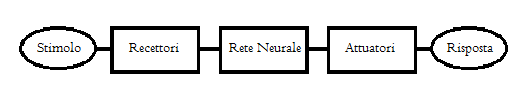
\includegraphics[width=0.7\linewidth]{IMMAGINI/GRAFOSISTNERV}
		\caption{}
		\label{fig: stadi sistema nervoso}
	\end{figure}
	
	
	
	
		Sono sistemi computazionali ispirati a processi biologici con le seguenti caratteristiche:  • formati da milioni di unità computazionali (neuroni) capaci di eseguire una somma pesata;  • elevato numero di connessioni pesate (sinapsi) tra le unità;  • altamente paralleli e non lineari;  • adattivi e addestrabili e l'apprendimento avviene attraverso la modifica dei pesi delle connessioni;  • tolleranti agli errori in quanto la memorizzazione avviene in modo diffuso;  • non c'è distinzione tra memoria e area di calcolo;  • capacità di generalizzazione: producono output ragionevoli con input mai incontrati prima durante l'apprendimento. 
		
		L'attivitàdella singola unitàèsemplice (funzione di trasferimento) e la potenza dei modello risiede nella configurazione delle connessioni (topologia e intensità).
		Partendo dalle unitàdi input, a cui vengono forniti i dati dei problema da risolvere, la computazione si propaga in parallelo nella rete fino alle unitàdi output, che forniscono il risultato.
		Una RN non viene programmata per eseguire una certa attività, ma addestrata (utilizzando un algoritmo di apprendimento automatico) mediante una serie di esempi della realtàda modellare
		
		
		
	Nel sistema nervoso esistono miliardi di neuroni (cellule nervose). Un neurone è formato da un corpo cellulare e da molti prolungamenti ramificati, detti dendriti, attraverso i quali il neurone riceve segnali elettrici da altri neuroni. Ogni neurone ha anche un prolungamento filamentoso chiamato assone, la cui lunghezza può variare da circa 1 cm a qualche metro. All’estremità l’assone si ramifica formando terminali attraverso i quali i segnali elettrici vengono trasmessi ad altre cellule (ad esempio ai dendriti di altri neuroni). Tra un terminale di un assone e la cellula ricevente esiste uno spazio. I segnali superano questo spazio per mezzo di sostanze chimiche dette neurotrasmettitori. Il punto di connessione tra terminale e dendrite è detto sinapsi. Un neurone si “attiva”, cioè trasmette un impulso elettrico lungo il suo assone quando si verifica una differenza di potenziale elettrico tra l’interno e l’esterno della cellula. L’impulso elettrico provoca la liberazione di un neurotrasmettitore dai terminali dell’assone, che a loro volta possono, ad esempio, influenzare altri neuroni. I neuroni biologici sono da 5 a 6 ordini di grandezza più lenti dei componenti elettronici convenzionali: un evento in un chip si verifica in alcuni nanosecondi (10-9 s) mentre un evento neurale in alcuni millisecondi (10-3 s). Il cervello umano è un calcolatore complesso, non lineare e parallelo. Pur essendo costituito da elementi di elaborazione molto semplici (i neuroni), è in grado di eseguire computazioni complesse, come il riconoscimento, la percezione e il controllo del movimento, molte volte più velocemente del più veloce degli attuali calcolatori. Il cervello è in grado di modificare le connessioni tra i neuroni in base all’esperienza acquisita, cioè è in grado di imparare. 
		
		
	 
		La corteccia celebrale è formata da circa 10 bilioni di neuroni e 60 trilioni di sinapsi. 
		ogni neurone ha velocità dell'ordine dei millisecondi, contro i nanosecondi dei chip in silicio; 
		l'efficienza energetica è di circa 10-16 J per operazione per secondo contro i 10-6 del migliore
		computer in uso oggi. 
		
		Un neurone è caratterizzato da:
		corpo cellulare: l'unità di calcolo (soma); 
		assone: linea di trasmissione in uscita; 
		dendriti: le zone recettive. 
		
		Il neurone ha il compito di fare una somma pesata degli ingressi e se il risultato supera un certo valore soglia produce un potenziale d'azione che viene inviato all'assone, altrimenti non fa nulla. 
		
		Il potenziale d'azione consiste in una scarica di impulsi elettrici e il motivo di ciò è che l'assone è molto lungo e fine, caratterizzato da alta resistenza elettrica e un voltaggio applicato ad un estremità decade in modo esponenziale con la distanza; inviando diversi impulsi elettrici questo problema di trasmissione viene evitato. 
		
		Le sinapsi sono unità funzionali dalla struttura elementare che gestisce le iterazioni tra neuroni. La sinapsi più comune è la sinapsi chimica che svolge le seguenti operazioni: 
		4
		• un processo presinaptico libera una sostanza trasmettitrice che si diffonde lungo la giunzione sinaptica tra 2 neuroni; • un processo postsinaptico azionato dalla sostanza trasmettitrice rigenera un segnale elettrico. 
		
		Quindi una sinapsi converte un segnale elettrico in chimico della presinapsi e poi da chimico a elettrico nella postsinapsi. 
		
		Ci sono 2 tipi di sinapsi: 1. eccitatorie: favoriscono la generazione di elettricità nel neurone postsinaptico; 2. inibitorie: inibiscono la generazione di elettricità nel neurone postsinaptico. 
		
		Pare che l'apprendimento avvenga attraverso variazioni nell'efficacia sinaptica di ogni sianpsi. 
		
		
		
		\section{Struttura e modello matematico}
		\section{Architettura}
		\section{Funzioni di attivazione}
	%FINE DEL PRIMO CAPITOLO
	
	\chapter{Feed Forward}
	\chapter{Ricorrenti}

\clearpage 
%\phantomsection 
\addcontentsline{toc}{section}{\refname}
\begin{thebibliography}{9} 
	\bibitem[1]{Lazzarini} Prof.ssa Lazzarini Beatrice, (2015), \emph{Introduzione alle reti neurali.}
	\bibitem[2]{Gambosi} Prof. Gambosi Giorgio, (2010), \emph{Reti neurali, note dal corso di Machine Learning.}
	\bibitem[3]{Labonia} Prof.ssa Labonia Laura, \emph{Storia delle reti neurali artificiali.}
	\bibitem[4]{Bicego} Prof. Bicego Manuele, \emph{Riconoscimento e recupero dell’informazione per bioinformatica. Reti neurali.}
	\bibitem[5]{Pioggia} Ing. Pioggia Giovanni, (2009), \emph{Modelli di sistemi fisiologici}
 \end{thebibliography}
	
\end{document}